\documentclass[10pt]{article}
\usepackage[preprint,nonatbib]{neurips_2025}
\usepackage[T1]{fontenc}
\usepackage{amsmath,amssymb,graphicx,booktabs,array}
\usepackage{hyperref,url,microtype}
\hypersetup{hidelinks,pdfauthor={Yangxiao Cai},pdfsubject={COMP6704 source fingerprint: 1ad8650adfb43f74b0beffe57dde1b0bca50f4a5efe94ad688fde58892385eb2}}
\makeatletter
\renewcommand{\@noticestring}{COMP6704 Individual Assignment, Fall 2026. Unconstrained Optimization.}
\makeatother
\newlength{\paperfigurewidth}
\title{Stationarity, Evaluation Cost, and Solution Quality\\ in Nonconvex Unconstrained Optimization}
\author{Yangxiao Cai  |  Student ID: 26023041r \\ COMP6704 Individual Assignment, Fall 2026 \\ Primary direction: Unconstrained Optimization}
\begin{document}
\maketitle
\begin{abstract}
We compare Armijo gradient descent (GD), safeguarded nonlinear conjugate gradient (CG), and BFGS on Rosenbrock and Rastrigin through 90 controlled CPU solves. Dimensions 2, 10, and 20 each use five paired initial points and fixed stopping criteria. In the recorded Windows reference run, 73/90 runs meet the gradient tolerance and 26/90 meet the global-objective tolerance: 47 meet only the gradient criterion, while 17 meet neither. On Rosenbrock, CG and BFGS attain the global-objective target in 14/15 and 12/15 cases; GD reaches the iteration cap in all 15 cases. On Rastrigin, 43/45 runs meet the gradient tolerance, but none meets the global-objective target. Endpoint diagnostics and comparisons conditional on CG and BFGS both meeting the global-objective target separate local convergence, evaluation cost, and final objective quality. Complete traces support this empirical distinction.

\end{abstract}
\setcounter{section}{0}
\section{Introduction and scope}
Smooth unconstrained optimization is a useful setting for studying how descent directions, line searches, curvature information, and stopping rules interact. It also exposes a practical ambiguity: software may report successful termination at a point with a small gradient even when its objective remains far from the global minimum. Comparing iteration counts alone can conceal both this difference in solution quality and the work spent rejecting trial steps.

This individual project belongs to Unconstrained Optimization. The variables range over all of real Euclidean space, and the objectives are nonconvex. The group project selected the Convex Optimization direction; the present investigation instead studies local algorithms outside convexity. Rosenbrock supplies a curved valley and coupled coordinates, while Rastrigin supplies many attraction basins and separable oscillations. Both have known global objective value zero, making stationarity and global-objective quality independently measurable \cite{ref7,ref8}.

Three questions guide the comparison. First, which methods reach the common gradient tolerance within a fixed accepted-update budget? Second, what function and gradient evaluation costs accompany their outcomes across dimensions and paired starts? Third, when termination is unsuccessful or non-global, what do the saved traces and endpoint curvature actually support? The design fixes the implementations and settings before comparing all 90 outcomes, including failures.

{\small Code availability. The PDF embeds \texttt{COMP6704\_reproducibility.zip} as a file attachment. Extract it through a PDF reader's attachment panel; README.md provides setup, verification, and reproduction commands.\par}

% Planned content page 2
\newpage
\setcounter{section}{1}
\section{Literature review and connection to the course}
Classical foundation. Nocedal and Wright \cite{ref1} organize smooth unconstrained methods around a search direction and an inexact line search. Their treatment connects first-order stationarity, descent, quasi-Newton curvature, and local convergence. These concepts provide the classroom framework here: an update can decrease the objective while remaining slow, and a necessary first-order condition becomes sufficient for global optimality only under additional structure such as convexity. Our nonconvex functions deliberately remove that sufficiency.

Step selection and memory. Armijo's early work \cite{ref2} established a sufficient-decrease approach to choosing step lengths. GD uses the current negative gradient, making its behavior easy to audit but sensitive to geometry. Nonlinear CG carries information from the preceding search direction. Gilbert and Nocedal \cite{ref3} analyze globally convergent CG variants with appropriate safeguards and line searches on smooth nonconvex problems. Such results depend on the precise variant and assumptions; they do not imply that an arbitrary Polak--Ribiere implementation or a positive \(\beta\) alone ensures descent. The PR+ implementation used here therefore warrants source-level identification.

Quasi-Newton methods. Fletcher's variable-metric development \cite{ref4} is part of the foundation of BFGS. BFGS learns curvature from successive displacements and gradient differences instead of forming an analytic Hessian. This can improve local progress, at the cost of matrix storage and updates. Positive-definite inverse-Hessian approximations yield descent directions in exact arithmetic, but neither this property nor a Wolfe line search certifies a global minimizer on a nonconvex objective. Implementation details and finite precision remain relevant when a solver stops near its tolerance.

Recent theory. Jin, Jiang, and Mokhtari \cite{ref5} obtain explicit non-asymptotic rates for BFGS with Armijo--Wolfe line search under strong convexity and smoothness; additional regularity supports stronger rate statements. Their analysis clarifies the gap between qualitative convergence and finite-iteration performance. Strong convexity is absent globally in our tests, so these rates provide context rather than a theorem for the recorded runs. Mannel \cite{ref6} studies a modified, globalized L-BFGS and Barzilai--Borwein framework for nonconvex unconstrained optimization, using cautious updates and conditions supporting stationarity of cluster points. This is a different algorithm from ordinary full-memory SciPy BFGS. Its relevance is that nonconvex guarantees require carefully designed safeguards, rather than a change of terminology.

\begingroup
\fontsize{8}{9.2}\selectfont
\setlength{\tabcolsep}{3pt}
\renewcommand{\arraystretch}{1.05}
\centering
\begin{tabular}{@{}>{\raggedright\arraybackslash}p{\dimexpr 0.28000000\linewidth-3.360000pt\relax}>{\raggedright\arraybackslash}p{\dimexpr 0.35000000\linewidth-4.200000pt\relax}>{\raggedright\arraybackslash}p{\dimexpr 0.37000000\linewidth-4.440000pt\relax}@{}}
\toprule
\textbf{Source / line of work} & \textbf{Relevance to this study} & \textbf{Boundary of the comparison} \\
\midrule
Armijo \cite{ref2}; textbook \cite{ref1} & Sufficient decrease; descent-lemma reasoning & Finite backtracking caps can terminate early \\
Gilbert--Nocedal \cite{ref3} & Nonlinear CG safeguards and nonconvex analysis & Identify the actual PR+ implementation \\
Jin et al. \cite{ref5}, 2024 & Finite-time BFGS analysis with inexact line search & Strong-convexity rates do not apply globally here \\
Mannel \cite{ref6}, 2025 & Nonconvex globalization of limited-memory methods & Modified L-BFGS is not the tested full BFGS \\
\bottomrule
\end{tabular}\par
\endgroup
\smallskip
Study position. The controlled comparison distinguishes satisfaction of the gradient criterion, objective quality, and evaluation cost using complete traces. Version-pinned SciPy documentation and source \cite{ref7} determine the implemented CG and BFGS behavior. Known optima and transparent benchmark geometry make discrepancies between success labels and objective quality directly measurable; Section 9 discusses the limits of this design.


% Planned content page 3
\newpage
\setcounter{section}{2}
\section{Formal problem and objective geometry}
We solve \(\min f(x)\) over \(x\in\mathbb{R}^d\), with d in \{2, 10, 20\}; no feasibility constraints or projections are imposed. Write \(g_k\) = \(\nabla f(x_k)\), use the Euclidean \texttt{norm} throughout, and denote the known global objective by \(f^\star=0\). The two benchmark models are

\setcounter{equation}{0}
\begin{equation}
\begin{aligned}
f_R(x)=\sum_{i=1}^{d-1}\left[100(x_{i+1}-x_i^2)^2+(1-x_i)^2\right]
\end{aligned}
\label{eq:models_R}
\end{equation}
\setcounter{equation}{1}
\begin{equation}
\begin{aligned}
f_A(x)=\sum_{i=1}^{d}\left[x_i^2+20\sin^2(\pi x_i)\right]
\end{aligned}
\label{eq:models_A}
\end{equation}
The Rastrigin expression is algebraically equivalent to \(10d+\sum_i[x_i^2-10\cos(2\pi x_i)]\) \cite{ref8}. The sine-squared form avoids cancellation between large constants near zero. Rosenbrock uses SciPy's \texttt{rosen} and \texttt{rosen\_der}; Rastrigin has the analytic derivative

\setcounter{equation}{2}
\begin{equation}
\begin{aligned}
\relax [\nabla f_A(x)]_i=2x_i+20\pi\sin(2\pi x_i)
\end{aligned}
\label{eq:gradients_A}
\end{equation}
For Rosenbrock, each term indexed by i contributes \(-400x_i(x_{i+1}-x_i^2)+2(x_i-1)\) to derivative component i and \(200(x_{i+1}-x_i^2)\) to component i+1. The implementation accumulates all adjacent contributions. Before solving, central differences at 12 nonstationary test points check both gradients, using \(h_i=10^{-6}\max(1,|x_i|)\) and componentwise absolute and relative tolerances \(10^{-5}\). All 12 checks pass; those checks are outside solver evaluation counts.

Known optima and nonconvexity. Both models are sums of nonnegative terms. Rosenbrock reaches zero only at the all-ones vector for d \(\geq\) 2; Rastrigin reaches zero only at the zero vector. In two-dimensional Rosenbrock, the Hessian at (0,1) is diag(-398,200), so the function is not convex. This point is not a saddle point: its gradient is (-2,200), which is nonzero. For Rastrigin the Hessian is diagonal with entries \(2+40\pi^2\cos(2\pi x_i)\); a coordinate equal to 1/2 yields negative curvature. Negative curvature at an arbitrary point establishes nonconvexity, not stationarity.

The coupled Rosenbrock valley makes curvature vary strongly with direction. Rastrigin is separable, yet its oscillatory terms produce many local basins; coordinatewise independence therefore does not make a local descent method a global solver. Both functions are smooth and coercive, so bounded objective sublevels are compact. Their gradients have suitable local Lipschitz bounds on bounded regions, but Rosenbrock's gradient is not globally Lipschitz over all of \(\mathbb{R}^d\). At the two-dimensional Rosenbrock global minimizer, the Hessian has eigenvalues approximately 0.39936 and 1001.60064, giving condition number about 2508. This local ill-conditioning is consistent with slow GD progress; it is not a rate estimate for the full nonlinear trajectory. These distinctions matter when stating descent guarantees.

\setcounter{section}{3}
\section{Algorithms and implementation}
\setcounter{section}{4}
\setcounter{subsection}{0}
\subsection{Gradient descent with Armijo backtracking}
\setcounter{equation}{3}
\begin{equation}
\begin{aligned}
g_k=\nabla f(x_k),\qquad x_{k+1}=x_k-\alpha_k g_k \\
f(x_k-\alpha_k g_k)\leq f(x_k)-c_1\alpha_k\|g_k\|_2^2
\end{aligned}
\label{eq:gd_armijo}
\end{equation}
GD is implemented directly. Every iteration starts again at \(\alpha_0\) = 1, halves the trial step with \(\tau\) = 0.5, and accepts the first point satisfying (4), with \(c_1\) = \(10^{-4}\). At most 50 reductions follow the initial trial, and the minimum step is \(10^{-12}\). A rejected trial never updates x. Nonfinite values, an unchanged floating-point point, and an exhausted line search receive explicit failure statuses. The accepted-update limit is 5000; all function calls at rejected trial points still count.


% Planned content page 4
\newpage
\setcounter{section}{4}
\setcounter{subsection}{1}
\subsection{Safeguarded nonlinear conjugate gradient}
\setcounter{equation}{4}
\begin{equation}
\begin{aligned}
p_0=-g_0,\qquad p_k=-g_k+\beta_k^{\mathrm{PR+}}p_{k-1}\quad(k\geq1) \\
\beta_k^{\mathrm{PR+}}=\max\left\{0,\frac{g_k^\top(g_k-g_{k-1})}{g_{k-1}^\top g_{k-1}}\right\}
\end{aligned}
\label{eq:cg}
\end{equation}
CG uses \texttt{scipy.optimize.minimize(method='CG')} with analytic gradients. Equation (5) is the PR+ direction recurrence, initialized with \(p_0=-g_0\) \cite{ref3,ref7}. SciPy 1.13.1 adds a sufficient-descent acceptance check for the proposed next direction: the inner product of the next direction and gradient must not exceed -0.01 times the squared gradient \texttt{norm}, unless the gradient target is already met. PR+ truncation alone does not guarantee this property. This safeguard is not a fixed periodic restart. Both SciPy methods use the strong-Wolfe conditions

\setcounter{equation}{5}
\begin{equation}
\begin{aligned}
f(x_{k+1})\leq f(x_k)+c_1\alpha_k g_k^\top p_k \\
|g_{k+1}^\top p_k|\leq c_2|g_k^\top p_k|,\qquad 0<c_1<c_2<1
\end{aligned}
\label{eq:wolfe}
\end{equation}
Here \(0<c_1=10^{-4}<c_2=0.4<1\). The same constants reduce one source of variation between CG and BFGS, although their search directions and internal trial sequences still differ. Function and gradient counts consequently remain necessary measurements.

\setcounter{section}{4}
\setcounter{subsection}{2}
\subsection{Full-memory BFGS}
BFGS uses \texttt{scipy.optimize.minimize(method='BFGS')}, \(p_k=-H_k g_k\), and \(H_0=I\). With displacement \(s_k\) and gradient change \(y_k\) as defined below, the inverse-Hessian update is \cite{ref1,ref4}

\setcounter{equation}{6}
\begin{equation}
\begin{aligned}
H_{k+1}=(I-\rho_k s_k y_k^\top)H_k(I-\rho_k y_k s_k^\top)+\rho_k s_k s_k^\top \\
s_k=x_{k+1}-x_k,\quad y_k=g_{k+1}-g_k,\quad\rho_k=(y_k^\top s_k)^{-1}
\end{aligned}
\label{eq:bfgs}
\end{equation}
\setcounter{section}{4}
\setcounter{subsection}{3}
\subsection{Ideal Armijo GD stationarity bound}
For GD, assume f is bounded below by \(f_{\inf}\) and its gradient is L-Lipschitz with one uniform constant L on all relevant trial segments. Coercivity bounds accepted iterates; bounded gradients there and trial steps no larger than one contain the trial segments in a compact region, where smoothness supplies such an L. The descent lemma makes any \(\alpha\leq2(1-c_1)/L\) sufficient for (4). With ideal unlimited backtracking from one, an accepted \(\alpha\) is at least the lower bound below. Summing (4) over K updates gives

\setcounter{equation}{7}
\begin{equation}
\begin{aligned}
\alpha_{\mathrm{low}}=\min\left\{1,\frac{2\tau(1-c_1)}{L}\right\}>0 \\
\min_{0\leq k<K}\|g_k\|_2^2\leq\frac{f(x_0)-f_{\inf}}{c_1\alpha_{\mathrm{low}}K}
\end{aligned}
\label{eq:gd_bound}
\end{equation}
Thus ideal Armijo GD has a standard \(\mathcal{O}(\epsilon^{-2})\) accepted-update bound for finding an iterate with gradient \texttt{norm} at most \(\epsilon\) under these assumptions. This is a stationarity result, not a global-optimality result. The actual finite iteration, trial, and minimum-step limits can stop a run before it reaches that target; the asymptotic statement does not override its recorded failure.

\setcounter{section}{4}
\setcounter{subsection}{4}
\subsection{BFGS curvature implication}
For a descent direction \(p_k\) and an accepted strong-Wolfe step, (6) gives the curvature inequality

\setcounter{equation}{8}
\begin{equation}
\begin{aligned}
s_k^\top y_k\geq\alpha_k(1-c_2)(-g_k^\top p_k)>0
\end{aligned}
\label{eq:curvature}
\end{equation}
In exact arithmetic, (7) therefore preserves positive definiteness from \(H_0\)=I, even when the true Hessian is indefinite. This curvature property does not ensure global optimality or prevent finite-precision failure. The strong-convexity rates in \cite{ref5} do not apply globally here; CG convergence likewise requires its line-search and regularity hypotheses.


% Planned content page 5
\newpage
\setcounter{section}{4}
\section{Experimental protocol, costs, and auditing}
\begingroup
\fontsize{8}{9.2}\selectfont
\setlength{\tabcolsep}{3pt}
\renewcommand{\arraystretch}{1.05}
\centering
\begin{tabular}{@{}>{\raggedright\arraybackslash}p{\dimexpr 0.22000000\linewidth-1.320000pt\relax}>{\raggedright\arraybackslash}p{\dimexpr 0.78000000\linewidth-4.680000pt\relax}@{}}
\toprule
\textbf{Component} & \textbf{Fixed protocol} \\
\midrule
Design & 2 functions x 3 dimensions x 5 paired starts x 3 methods = 90 solves \\
Initialization & Seed 20261105; \texttt{PCG64} with \texttt{SeedSequence}([seed, objective\_index, d]); coordinates uniform on [-2,2] for Rosenbrock and [-3,3] for Rastrigin \\
Stopping & Euclidean gradient \texttt{norm} \(\leq\) \(10^{-6}\); at most 5000 accepted updates \\
SciPy options & CG/BFGS: \(c_1\)=\(10^{-4}\), \(c_2\)=0.4, \texttt{norm}=2, \texttt{gtol}=\(10^{-6}\), \texttt{maxiter}=5000. BFGS: \(H_0=I\), \texttt{xrtol}=0; default \(c_2\)=0.9 is overridden. No analytic Hessian or damping. \\
Arithmetic / environment & \texttt{float64}; Python 3.12.8, NumPy 1.26.4, SciPy 1.13.1; Windows 11; sequential CPU solves; BLAS/OpenMP thread variables set to 1 \\
Hardware record & Intel64 Family 6 Model 191 Stepping 2; 24 logical CPUs reported; no GPU used \\
Independent outcomes & Native solver status; S: finite result and \(\|\nabla f\|_2\) \(\leq\) \(10^{-6}\); G: finite result and \(|f-f^\star|\) \(\leq\) \(10^{-6}\) \\
\bottomrule
\end{tabular}\par
\endgroup
\smallskip
The intervals above generate initial points only; they do not constrain subsequent iterates. Each function-dimension pair has its own random stream, and each of its five saved starts is shared across methods. This pairing controls starting difficulty without asserting that five points represent all possible initializations. The two tolerances define different questions. Native \texttt{solver\_success} and S happen to agree for these 90 runs, but remain distinct fields; G is a known-objective target rather than a mathematical certificate of exact optimality.

Evaluation accounting. A wrapper counts every actual raw objective and gradient call made by a solver, including rejected line-search trials and trials in a failed terminal search. Calls avoided by SciPy's cache are not invented. The wrapper counts must equal SciPy's returned \texttt{nfev}/\texttt{njev}. Callbacks only copy accepted coordinates and snapshot counters; they do not reevaluate f or g. Each trace contains an initial event with counters zero, one event per accepted update, and a terminal event. Initial plot diagnostics and every recorded objective/gradient \texttt{norm} are filled offline from raw functions, outside the counters and timer. Thus the initial point can appear at \texttt{nfev}=0 without making the solver's own initial evaluation free.

The study records 80,605 events: 80,425 accepted updates and 180 initial/terminal events. Solver time covers evaluations, updates, and event capture, excluding imports, offline diagnostics, file I/O, and plotting. The sum of measured solver times is 26.915 s, rather than total pipeline wall time. Timing is secondary because these small problems are sensitive to Python, callback, and scheduling overhead. Figures stop at each actual endpoint; no curve is extended after termination, and log-display floors never change raw values.

\begingroup
\fontsize{8}{9.2}\selectfont
\setlength{\tabcolsep}{3pt}
\renewcommand{\arraystretch}{1.05}
\centering
\begin{tabular}{@{}>{\raggedright\arraybackslash}p{\dimexpr 0.16000000\linewidth-1.920000pt\relax}>{\raggedright\arraybackslash}p{\dimexpr 0.67000000\linewidth-8.040000pt\relax}>{\raggedright\arraybackslash}p{\dimexpr 0.17000000\linewidth-2.040000pt\relax}@{}}
\toprule
\textbf{Method} & \textbf{Direction / update arithmetic} & \textbf{Solver state} \\
\midrule
GD & \(\mathcal{O}(d)\) per direction; line-search calls additional & \(\mathcal{O}(d)\) \\
PR+ CG & \(\mathcal{O}(d)\) per direction; line-search calls additional & \(\mathcal{O}(d)\) \\
BFGS & \(\mathcal{O}(d^{2})\) direction; standard low-rank update \(\mathcal{O}(d^{2})\); tested SciPy dense-product update \(\mathcal{O}(d^{3})\)* & \(\mathcal{O}(d^{2})\) \\
\bottomrule
\end{tabular}\par
\endgroup
\smallskip
{\small\itshape Table 1. Algorithmic work excludes objective/gradient calls, each \(\mathcal{O}(d)\) for these models. *SciPy 1.13.1 forms A1 @ H @ A2 using generic dense products \cite{ref7}; \(\mathcal{O}(d^{3})\) uses conventional dense arithmetic, not an empirical scaling fit. Storing K d-dimensional trace points adds \(\mathcal{O}(Kd)\) space for every method.\par}\smallskip
Audit checks cover pairings, trace structure, monotone counters, GD sufficient decrease, endpoints, native counts, and source hashes. All 50 unit tests and the independent full-study validator pass.


% Planned content page 6
\newpage
\setcounter{section}{5}
\section{Results: Rosenbrock}
\begingroup
\fontsize{8}{9.2}\selectfont
\setlength{\tabcolsep}{3pt}
\renewcommand{\arraystretch}{1.05}
\centering
\begin{tabular}{@{}>{\raggedright\arraybackslash}p{\dimexpr 0.04500000\linewidth-1.620000pt\relax}>{\raggedright\arraybackslash}p{\dimexpr 0.10000000\linewidth-3.600000pt\relax}>{\raggedright\arraybackslash}p{\dimexpr 0.06500000\linewidth-2.340000pt\relax}>{\raggedright\arraybackslash}p{\dimexpr 0.10500000\linewidth-3.780000pt\relax}>{\raggedright\arraybackslash}p{\dimexpr 0.20500000\linewidth-7.380000pt\relax}>{\raggedright\arraybackslash}p{\dimexpr 0.18000000\linewidth-6.480000pt\relax}>{\raggedright\arraybackslash}p{\dimexpr 0.30000000\linewidth-10.800000pt\relax}@{}}
\toprule
\textbf{d} & \textbf{Method} & \textbf{S/G} & \textbf{Updates\newline{}median} & \textbf{\texttt{nfev}\newline{}median [range]} & \textbf{\texttt{njev}\newline{}median [range]} & \textbf{Final f\newline{}median [range]} \\
\midrule
2 & GD & 0/0 & 5000 & 49290\newline{}[49090, 51127] & 5001\newline{}[5001, 5001] & \(4.64\times10^{-6}\)\newline{}[\(3.35\times10^{-6}\), \(5.07\times10^{-5}\)] \\
2 & CG & 5/5 & 23 & 56\newline{}[32, 72] & 56\newline{}[32, 72] & \(2.49\times10^{-16}\)\newline{}[\(4.24\times10^{-20}\), \(3.03\times10^{-13}\)] \\
2 & BFGS & 5/5 & 25 & 48\newline{}[20, 58] & 48\newline{}[20, 58] & \(1.33\times10^{-17}\)\newline{}[\(8.99\times10^{-21}\), \(8.49\times10^{-15}\)] \\
10 & GD & 0/0 & 5000 & 53100\newline{}[53063, 53339] & 5001\newline{}[5001, 5001] & \(4.91\times10^{-4}\)\newline{}[\(4.14\times10^{-4}\), \(4.99\times10^{-4}\)] \\
10 & CG & 5/4 & 249 & 434\newline{}[282, 553] & 434\newline{}[282, 553] & \(9.47\times10^{-14}\)\newline{}[\(2.11\times10^{-14}\), 3.99] \\
10 & BFGS & 5/3 & 70 & 114\newline{}[100, 146] & 114\newline{}[100, 146] & \(3.08\times10^{-17}\)\newline{}[\(2.80\times10^{-18}\), 3.99] \\
20 & GD & 0/0 & 5000 & 53289\newline{}[53071, 53376] & 5001\newline{}[5001, 5001] & 0.00353\newline{}[0.00339, 0.004] \\
20 & CG & 5/5 & 444 & 709\newline{}[482, 900] & 709\newline{}[482, 900] & \(1.10\times10^{-13}\)\newline{}[\(5.87\times10^{-16}\), \(1.35\times10^{-13}\)] \\
20 & BFGS & 5/4 & 110 & 175\newline{}[166, 203] & 175\newline{}[166, 203] & \(3.72\times10^{-16}\)\newline{}[\(4.74\times10^{-18}\), 3.99] \\
\bottomrule
\end{tabular}\par
\endgroup
\smallskip
{\small\itshape Table 2. Rosenbrock, five starts in every row. S and G are counts out of five, not a ratio. Ranges are minima and maxima; failed runs remain included. Complete update and time ranges are in \texttt{grouped\_results.csv}. Scientific notation is rounded only for display.\par}\smallskip
\begingroup
\setlength{\paperfigurewidth}{507pt}
\ifdim\paperfigurewidth>\linewidth\setlength{\paperfigurewidth}{\linewidth}\fi
\noindent\makebox[\linewidth][c]{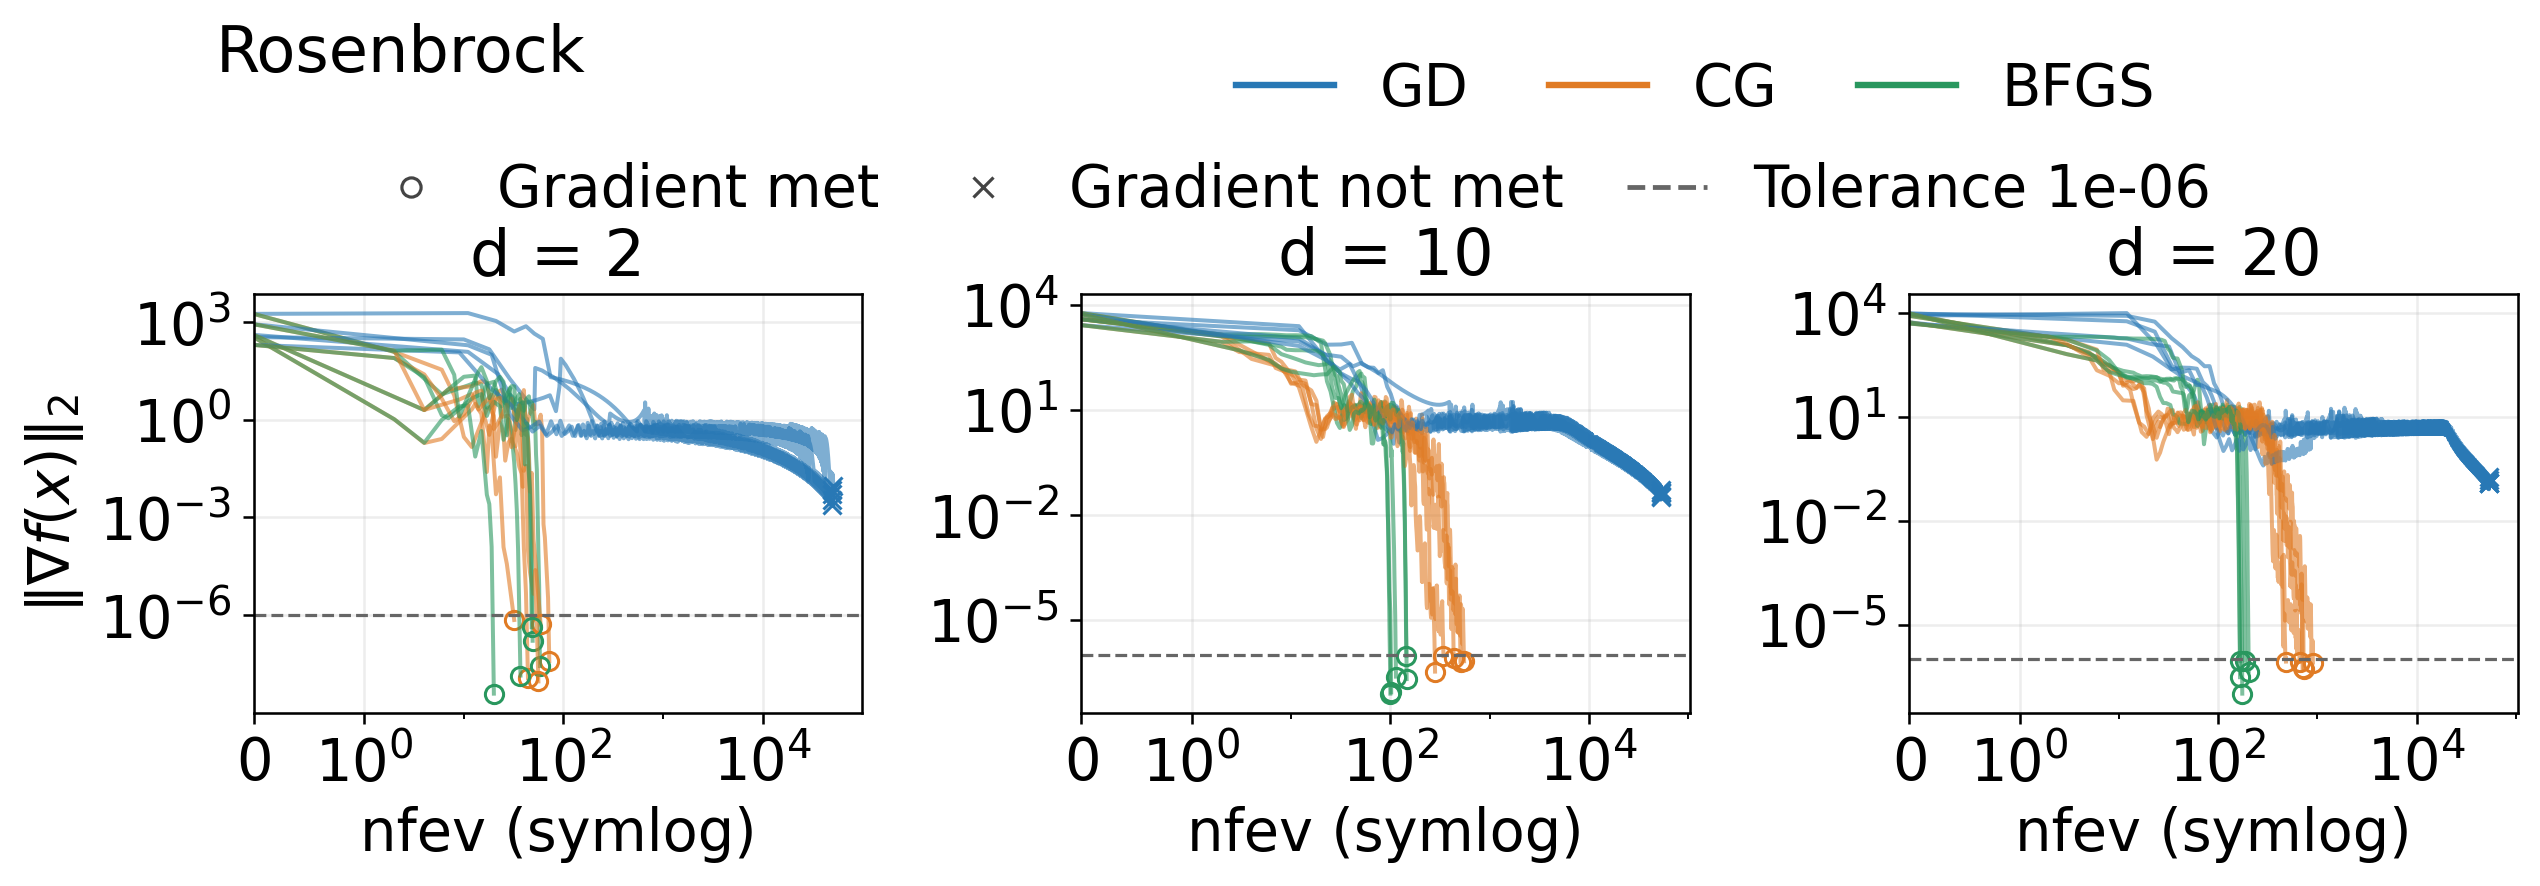
\includegraphics[width=\paperfigurewidth,height=185pt,keepaspectratio]{../assets/paper_rosenbrock_convergence.png}}\par
\endgroup
{\small\itshape Figure 1. Gradient \texttt{norm} against cumulative function evaluations for all five starts in each dimension. Colors denote methods; circles meet S and crosses do not. The x-axis is \texttt{symlog} with a linear region at zero; each curve stops at termination. The horizontal dashed line is \(10^{-6}\).\par}\smallskip
Budget and convergence. CG and BFGS meet the gradient criterion in all 15 Rosenbrock runs each; GD meets it in none. Every GD run accepts all 5000 permitted updates, with no failed line search. The final gradient medians are \(5.31\times10^{-3}\), \(4.30\times10^{-2}\), and \(1.26\times10^{-1}\) at d=2,10,20, well above tolerance. Accepted-step medians are 1/512, 1/1024, and 1/1024, while median trial counts per accepted step are 10, 11, and 11. Their large function counts reflect repeated trial rejection as well as slow progress in the valley. The geometry and reset-to-one policy offer a plausible explanation; this study has no ablation to isolate their causal contributions.


% Planned content page 7
\newpage
\setcounter{section}{6}
\section{Results: Rastrigin}
\begingroup
\fontsize{8}{9.2}\selectfont
\setlength{\tabcolsep}{3pt}
\renewcommand{\arraystretch}{1.05}
\centering
\begin{tabular}{@{}>{\raggedright\arraybackslash}p{\dimexpr 0.04500000\linewidth-1.620000pt\relax}>{\raggedright\arraybackslash}p{\dimexpr 0.10000000\linewidth-3.600000pt\relax}>{\raggedright\arraybackslash}p{\dimexpr 0.06500000\linewidth-2.340000pt\relax}>{\raggedright\arraybackslash}p{\dimexpr 0.10500000\linewidth-3.780000pt\relax}>{\raggedright\arraybackslash}p{\dimexpr 0.20500000\linewidth-7.380000pt\relax}>{\raggedright\arraybackslash}p{\dimexpr 0.18000000\linewidth-6.480000pt\relax}>{\raggedright\arraybackslash}p{\dimexpr 0.30000000\linewidth-10.800000pt\relax}@{}}
\toprule
\textbf{d} & \textbf{Method} & \textbf{S/G} & \textbf{Updates\newline{}median} & \textbf{\texttt{nfev}\newline{}median [range]} & \textbf{\texttt{njev}\newline{}median [range]} & \textbf{Final f\newline{}median [range]} \\
\midrule
2 & GD & 5/0 & 31 & 276\newline{}[249, 313] & 32\newline{}[29, 37] & 4.97\newline{}[0.995, 12.9] \\
2 & CG & 5/0 & 7 & 19\newline{}[10, 24] & 19\newline{}[10, 24] & 9.95\newline{}[3.98, 16.9] \\
2 & BFGS & 5/0 & 6 & 12\newline{}[9, 16] & 12\newline{}[9, 16] & 9.95\newline{}[3.98, 16.9] \\
10 & GD & 5/0 & 34 & 305\newline{}[288, 312] & 35\newline{}[33, 36] & 35.8\newline{}[25.9, 37.8] \\
10 & CG & 5/0 & 9 & 19\newline{}[14, 24] & 19\newline{}[14, 24] & 27.9\newline{}[23.9, 37.8] \\
10 & BFGS & 5/0 & 20 & 39\newline{}[32, 43] & 39\newline{}[32, 43] & 27.9\newline{}[23.9, 37.8] \\
20 & GD & 5/0 & 34 & 305\newline{}[293, 312] & 35\newline{}[34, 36] & 64.7\newline{}[41.8, 126] \\
20 & CG & 5/0 & 9 & 19\newline{}[15, 22] & 19\newline{}[15, 22] & 63.7\newline{}[41.8, 69.6] \\
20 & BFGS & 3/0 & 26 & 86\newline{}[45, 117] & 86\newline{}[45, 105] & 62.7\newline{}[41.8, 68.7] \\
\bottomrule
\end{tabular}\par
\endgroup
\smallskip
{\small\itshape Table 3. Rastrigin uses the same definitions and all-run convention as Table 2. In the final row, \texttt{nfev} and \texttt{njev} have equal medians but different ranges because one terminal search adds unequal function and gradient counts.\par}\smallskip
Stationarity and objective quality separate sharply. GD and CG each meet S in 15/15 runs; BFGS meets S in 13/15. None of the 45 runs meets G. Hence 43 runs meet the gradient criterion while missing the global-objective target. Across each dimension, CG uses fewer function evaluations than GD: medians 19,19,19 versus 276,305,305. BFGS's corresponding medians are 12,39,86. These counts describe function evaluations to the observed endpoints; differing final objective values prevent an equal-quality cost comparison.

The paired final objectives in Figure 2 show how rankings depend on the outcome. At d=2, GD obtains a lower f than both other methods on four of the five starts, despite using more function evaluations. On start 1 it returns f=0.994959 with 313 function evaluations, compared with CG's 4.974790 using 24 and BFGS's 7.959662 using 10. All three methods meet the gradient criterion. For this starting point, GD achieves the lowest final objective value but requires the most function evaluations. Raw Rastrigin objectives add contributions across coordinates; their increase across dimensions alone is not evidence of worsening per-coordinate quality.

\setcounter{section}{7}
\setcounter{subsection}{0}
\subsection{The two BFGS precision-loss terminations}
\begingroup
\fontsize{8}{9.2}\selectfont
\setlength{\tabcolsep}{3pt}
\renewcommand{\arraystretch}{1.05}
\centering
\begin{tabular}{@{}>{\raggedright\arraybackslash}p{\dimexpr 0.14000000\linewidth-3.360000pt\relax}>{\raggedright\arraybackslash}p{\dimexpr 0.13000000\linewidth-3.120000pt\relax}>{\raggedright\arraybackslash}p{\dimexpr 0.20000000\linewidth-4.800000pt\relax}>{\raggedright\arraybackslash}p{\dimexpr 0.28000000\linewidth-6.720000pt\relax}>{\raggedright\arraybackslash}p{\dimexpr 0.25000000\linewidth-6.000000pt\relax}@{}}
\toprule
\textbf{20D start} & \textbf{Updates} & \textbf{\texttt{nfev} / \texttt{njev}} & \textbf{Final gradient \texttt{norm}} & \textbf{Final f} \\
\midrule
3 & 26 & 117 / 105 & \(8.73821\times10^{-6}\) & 41.78821486 \\
4 & 21 & 45 / 45 & \(1.00023457\times10^{-6}\) & 64.67220759 \\
\bottomrule
\end{tabular}\par
\endgroup
\smallskip
Both retain SciPy status=2 and its precision-loss message. At start 3 the last accepted event has counts 59/59; the terminal event adds 58 function and 46 gradient evaluations without accepting a new point. This directly exposes unsuccessful terminal trial work that iteration counts omit. At start 4 there are no extra terminal calls, and the last accepted objective change rounds to zero. Its final gradient \texttt{norm} is only 0.02346\% above the threshold, but it remains a failure under the fixed rule. Relaxing the threshold after seeing the result would change the protocol.

The common message does not uniquely identify an internal mechanism for each run. Failed line-search progress and finite-precision resolution are consistent with the saved evidence, but the traces do not expose every internal scalar. The analytic derivations and independent checks provide no evidence of a gradient implementation error. Finite checks do not exclude every numerical problem. Both outcomes are included in the final row of Table 3 and shown as crosses in Figure 2.


% Planned content page 8
\newpage
\setcounter{section}{7}
\section{Paired outcomes and endpoint interpretation}
\begingroup
\setlength{\paperfigurewidth}{507pt}
\ifdim\paperfigurewidth>\linewidth\setlength{\paperfigurewidth}{\linewidth}\fi
\noindent\makebox[\linewidth][c]{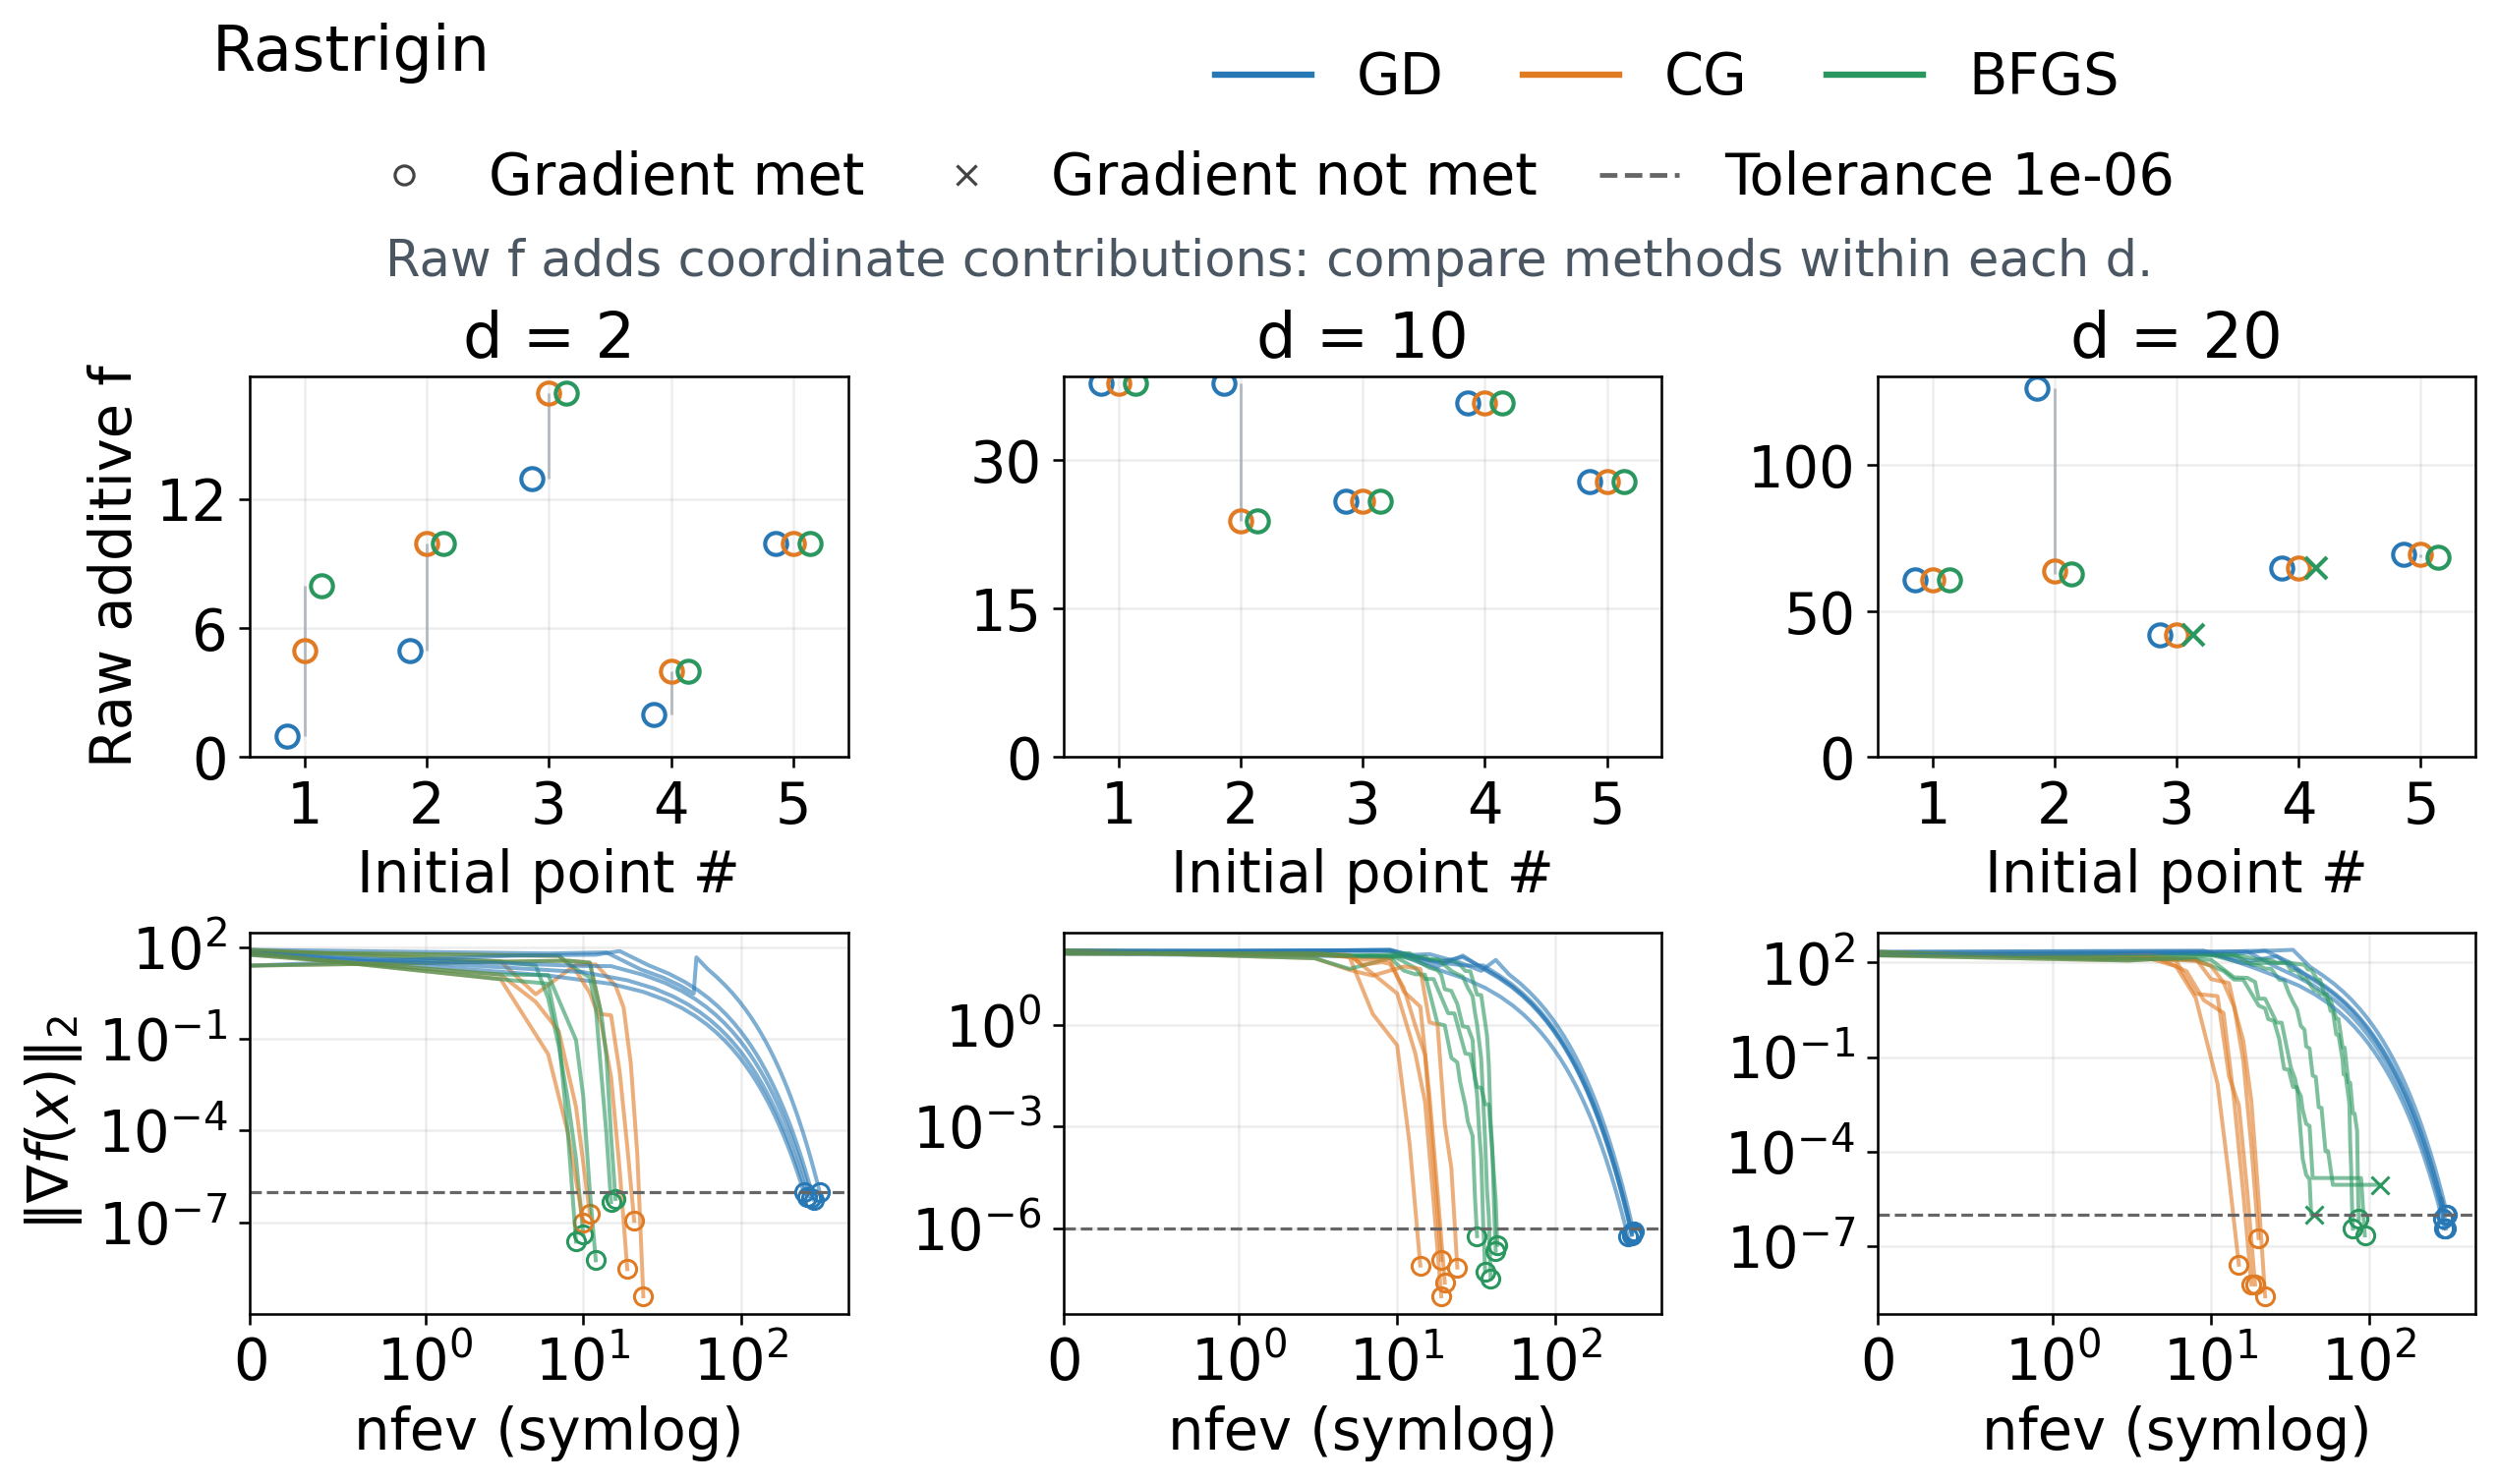
\includegraphics[width=\paperfigurewidth,height=318pt,keepaspectratio]{../assets/paper_rastrigin_quality_convergence.png}}\par
\endgroup
{\small\itshape Figure 2. All Rastrigin starts. Top: final raw f, with faint vertical segments connecting the range of three outcomes for each shared start. Bottom: gradient \texttt{norm} against cumulative \texttt{nfev}, with \texttt{symlog} x and log y. Colors denote methods; circles meet S and crosses do not. Compare objective quality within each dimension because f is additive. Curves end at their true termination, including unsuccessful runs.\par}\smallskip
\setcounter{section}{8}
\setcounter{subsection}{0}
\subsection{Non-global Rosenbrock endpoints}
\begingroup
\fontsize{8}{9.2}\selectfont
\setlength{\tabcolsep}{3pt}
\renewcommand{\arraystretch}{1.05}
\centering
\begin{tabular}{@{}>{\raggedright\arraybackslash}p{\dimexpr 0.28000000\linewidth-5.040000pt\relax}>{\raggedright\arraybackslash}p{\dimexpr 0.22000000\linewidth-3.960000pt\relax}>{\raggedright\arraybackslash}p{\dimexpr 0.20000000\linewidth-3.600000pt\relax}>{\raggedright\arraybackslash}p{\dimexpr 0.30000000\linewidth-5.400000pt\relax}@{}}
\toprule
\textbf{d / start / method} & \textbf{Final f} & \textbf{Gradient \texttt{norm}} & \textbf{Minimum Hessian eigenvalue} \\
\midrule
10 / 4 / CG & 3.9865791123 & \(9.56589\times10^{-7}\) & 0.501273 \\
10 / 4 / BFGS & 3.9865791123 & \(9.63817\times10^{-7}\) & 0.501273 \\
10 / 5 / BFGS & 3.9865791123 & \(8.78814\times10^{-8}\) & 0.501273 \\
20 / 1 / BFGS & 3.9866238543 & \(4.44622\times10^{-7}\) & 0.498755 \\
\bottomrule
\end{tabular}\par
\endgroup
\smallskip
{\small\itshape Table 4. The four Rosenbrock endpoints meeting S but missing G. Hessian spectra are computed offline and excluded from solve time and evaluation counts.\par}\smallskip
These four endpoints explain why 30 Rosenbrock runs meet the gradient criterion but only 26 meet the global-objective target. Positive numerical Hessian eigenvalues together with small gradients support the interpretation that the solvers finish near non-global local minima. At an approximate point, those quantities are numerical evidence, not an exact proof of a stationary local minimizer. Several methods can therefore converge convincingly while legitimately differing from the known global optimum. The contrast with GD's 15 budget-exhausted runs also separates convergence to a different basin from failure to reach stationarity within the budget.

Evaluation cost at comparable quality. BFGS's \texttt{nfev} medians rise from 48 to 114 to 175, while CG's rise from 56 to 434 to 709. Different counts of runs meeting G prevent an equal-quality comparison of these unconditional medians. Restricting to shared initial points for which both methods meet G leaves 5, 3, and 4 pairs for d=2,10,20; the median ratios of function evaluations, \texttt{nfev}(CG)/\texttt{nfev}(BFGS), are 1.24, 2.97, and 3.91. These median ratios favor BFGS in function evaluations; they do not measure wall time or describe starts where either method misses G. CG meets G in 14/15 runs overall versus BFGS in 12/15.


% Planned content page 9
\newpage
\setcounter{section}{8}
\section{Discussion, limitations, and reproducibility}
Interpretation of the three questions. First, in the recorded Windows reference run, 73/90 runs meet the common gradient criterion, with failures concentrated in Rosenbrock GD and two 20D Rastrigin BFGS runs. Second, function and gradient counts reveal costs hidden by accepted-update counts; the terminal 58/46 extra calls are a concrete example. The median ratios favor BFGS in function evaluations on the selected Rosenbrock pairs where both methods meet G, whereas CG uses fewer function evaluations than GD to its observed Rastrigin stationary endpoints. Third, final f and endpoint diagnostics show that meeting the gradient criterion does not imply meeting the global-objective target: 47 runs meet S while missing G. These observations connect descent and curvature concepts from the course to actual solver behavior.

Limits of the evidence. The study includes only two synthetic functions, three dimensions up to 20, and five fixed starts per setting. Its observed fractions are not estimated population success probabilities. Dimensions and changing random starts vary together, so trends across dimensions are descriptive. The experiment neither establishes asymptotic scaling nor measures the practical memory limit of BFGS. A single implementation and one set of line-search constants also cannot isolate the effects of direction, step selection, initialization, tolerance, and numerical safeguards. Millisecond timings do not justify a universal fastest-method claim, and conditioning cost ratios on both methods attaining G creates an explicitly selected subset.

Platform scope. The tables describe the recorded Windows run. Pinning NumPy and SciPy versions does not guarantee identical floating-point paths across operating systems, Python builds, processors, or linked numerical libraries. Small arithmetic differences can change line-search decisions, evaluation counts, and classifications near the strict \(10^{-6}\) threshold. A different execution path does not, by itself, invalidate the saved Windows records. Such differences require trace-level diagnosis; this study does not isolate a platform-specific cause.

Useful follow-up work would vary GD's initial trial-step policy under the same starts, sweep the stopping tolerance and iteration budget, and compare damped or limited-memory quasi-Newton variants using a larger test collection. Multi-start global search would address basin selection but would answer a different question from this fixed local-method comparison. A real-data smooth objective would improve external relevance while usually removing access to a known global optimum. These are future experiments, not results claimed here.

\setcounter{section}{9}
\setcounter{subsection}{0}
\subsection{Reproducibility and access}
The archive's README gives file access, exact commands, and audit scopes. Historical Windows-to-Windows comparison records are labelled separately from the archived unit tests and read-only data/source checks. These records establish neither a new formal experiment nor cross-platform numerical identity.

\setcounter{section}{9}
\section{Conclusion}
Under the fixed protocol, convergence to a small-gradient point did not imply a small global-objective gap. Rosenbrock favored CG and BFGS over this GD configuration within the iteration budget, but both sometimes reached non-global near-stationary points. On Rastrigin, all global-objective targets were missed despite 43/45 runs meeting the gradient criterion; GD occasionally obtained better objective values while using more function evaluations. The two BFGS precision-loss terminations were retained, including one just above tolerance. These results support separate reporting of stationarity, objective quality, costs, and failure modes.


% Planned content page 10
\newpage
\begin{thebibliography}{99}
\small\raggedright
\setlength{\itemsep}{2pt}
\bibitem{ref1}J. Nocedal and S. J. Wright. Numerical Optimization, 2nd ed. Springer, 2006. DOI: 10.1007/978-0-387-40065-5. \url{https://link.springer.com/book/10.1007/978-0-387-40065-5}
\bibitem{ref2}L. Armijo. Minimization of functions having Lipschitz continuous first partial derivatives. Pacific Journal of Mathematics, 16(1):1--3, 1966. \url{https://msp.org/pjm/1966/16-1/pjm-v16-n1-p01-p.pdf}
\bibitem{ref3}J. C. Gilbert and J. Nocedal. Global convergence properties of conjugate gradient methods for optimization. SIAM Journal on Optimization, 2(1):21--42, 1992. DOI: 10.1137/0802003. \url{https://doi.org/10.1137/0802003}
\bibitem{ref4}R. Fletcher. A new approach to variable metric algorithms. The Computer Journal, 13(3):317--322, 1970. DOI: 10.1093/comjnl/13.3.317. \url{https://doi.org/10.1093/comjnl/13.3.317}
\bibitem{ref5}Q. Jin, R. Jiang, and A. Mokhtari. Non-asymptotic global convergence analysis of BFGS with the Armijo-Wolfe line search. Advances in Neural Information Processing Systems 37:16810--16851, 2024. DOI: 10.52202/079017-0536. Author version: arXiv:2404.16731, revised January 8, 2025. \url{https://arxiv.org/abs/2404.16731}
\bibitem{ref6}F. Mannel. A globalization of L-BFGS and the Barzilai--Borwein method for nonconvex unconstrained optimization. Journal of Optimization Theory and Applications, 204, Article 47, 2025. DOI: 10.1007/s10957-024-02565-5. \url{https://link.springer.com/article/10.1007/s10957-024-02565-5}
\bibitem{ref7}SciPy developers. SciPy 1.13.1: minimize-CG and minimize-BFGS reference documentation and optimization tutorial; scipy/optimize/\_optimize.py, tag v1.13.1. Version-specific implementation and stopping/line-search options. Accessed November 5, 2026. \url{https://github.com/scipy/scipy/blob/v1.13.1/scipy/optimize/_optimize.py}
\bibitem{ref8}S. Surjanovic and D. Bingham. Virtual Library of Simulation Experiments: Test Functions and Datasets---Rastrigin Function. Simon Fraser University. Accessed November 5, 2026. \url{https://www.sfu.ca/~ssurjano/rastr.html}
\end{thebibliography}
{\small Version-specific option references supporting \cite{ref7}:\par}
{\small\raggedright CG documentation: \url{https://docs.scipy.org/doc/scipy-1.13.1/reference/optimize.minimize-cg.html}\par}
{\small\raggedright BFGS documentation: \url{https://docs.scipy.org/doc/scipy-1.13.1/reference/optimize.minimize-bfgs.html}\par}
{\small The course page limit includes this reference list. The PDF uses the official NeurIPS 2025 style with a course-specific notice.\par}
\end{document}
